\documentclass[11pt]{article}
\usepackage{graphicx,listings, amsmath, hyperref}
\graphicspath{ {./images/} }
\title{\textbf{IoT Final Project 2023 - Project 1}}
\author{
  Pasquale Castiglione\\
	\texttt{10657816}
  \and
  Lorenzo Campana\\
  \texttt{10605775}
}
\date{}
\begin{document}
\maketitle
\section*{mqtt.h}
The struct mqtt\_msg is used to define the message format to be sent between nodes. It contains the following attributes:
\begin{itemize}
  \item \texttt{type}
  \item \texttt{ID} (sender Node ID)
  \item \texttt{topic}
  \item \texttt{payload}
  \item \texttt{seq}, 32-bit number, used to identify a specific msg-ack sequence
\end{itemize}

\section*{mqttC.nc}
\subsection*{Variables}
\begin{itemize}
\item{\textbf{\texttt{locked}:}}\\
This boolean variable is used to indicate whether a message sending operation is currently in progress. When a message is being sent, this variable is set to TRUE, preventing further message sending until the current operation completes.
\item{\textbf{\texttt{time\_delays[N\_CLIENTS]}:}}\\
This array holds time delay values associated with each client ID. It's used for setting specific time delays before certain actions occur for each client.
\item{\textbf{\texttt{n\_subscription\_sim[N\_CLIENTS]}:}}\\
This array holds the number of remaining subscriptions each client needs to make. It's decremented as clients subscribe to topics.
\item{\textbf{\texttt{subscribed\_sim[N\_CLIENTS][N\_TOPICS]}:}}\\
This 2D array indicates whether a client is subscribed to a particular topic. It's used to track the subscription status of each client for different topics.
\item{\textbf{\texttt{panc\_table}:}}\\
This structure represents the table used to keep track of client connections and topic subscriptions.
\item{\textbf{\texttt{conn\_ack\_wait}:}}\\
This variable defines the initial waiting time for a CONNACK acknowledgment response from the broker. 
\item{\textbf{\texttt{sub\_ack\_wait}:}}\\
This variable defines the initial waiting time for a SUBACK acknowledgment response from the broker.
\item{\textbf{\texttt{waiting\_CONNACK}:}}\\
This structure is used to track the status and sequence number of the CONNECT acknowledgment response that the client is waiting for.
\item{\textbf{\texttt{waiting\_SUBACK}:}}\\
Similarly to \texttt{waiting\_CONNACK}, this structure tracks the status and sequence number of the SUBACK acknowledgment response that the client is waiting for.
\item{\textbf{\texttt{queued\_sub\_topic}:}}\\
This variable holds the topic that is currently queued for subscription. It's used to ensure that the correct topic is subscribed to after a timer event fires.

\end{itemize}

\subsection*{Functions}
\begin{itemize}
\item{\textbf{\texttt{init\_panc\_table}:}}\\
Initializes the Panc table structure to track client connections and subscriptions.
\item{\textbf{\texttt{send\_connect\_to\_PANC}:}}\\
Sends a CONNECT message to the PAN Coordinator to establish a connection.
\item{\textbf{\texttt{send\_subscribe}:}}\\
Sends a SUBSCRIBE message to the PAN Coordinator to subscribe to a specified topic.
\item{\textbf{\texttt{send\_publish}:}}
Sends a PUBLISH message to the PAN Coordinator to publish on a specified topic.
\item{\textbf{\texttt{create\_connection}:}}\\
Handles the creation of a connection and sends a CONNACK response to the client.
\item{\textbf{\texttt{create\_subscription}:}}\\
Handles the creation of a subscription and sends a SUBACK response to the client.
\item{\textbf{\texttt{forward\_publish}:}}\\
Forwards PUBLISH messages to subscribed clients.
\item{\textbf{\texttt{isConnected}:}}\\
Checks if a specific client is connected based on the Panc table.
\item{\textbf{\texttt{isSubscribed}:}}\\
Checks if a specific client is subscribed to a topic based on the Panc table.
\end{itemize}

\subsection*{Timers}
\begin{itemize}
\item{\textbf{\texttt{Timer0}:}}\\
Initiates the process of sending a CONNECT message to establis a connection.
\item{\textbf{\texttt{Timer\_wait\_CONNACK}:}}\\
Handles timeouts and retries for waiting for a CONNACK response.
\item{\textbf{\texttt{Timer\_wait\_SUBACK}:}}\\
Handles timeouts and retries for waiting for a SUBACK response.
\item{\textbf{\texttt{Timer\_SUB}:}}\\
Initiates the process of sending a SUBSCRIBE message to subscribe to a topic.
\item{\textbf{\texttt{Timer\_PUB}:}}\\
Initiates the process of sending a PUBLISH message.
\end{itemize}

\subsection*{Receive Event}
Received messages are handled according to their type:
\subsubsection*{PANC}
\begin{itemize}
\item{\textbf{\texttt{CONNECT Message}:}}\\
The handler calls the \texttt{create\_connection} function, which updates the texttt{Panc\_table} to mark the client as connected and sends a CONNACK acknowledgment back to the client.
The acknowledgment confirms the successful establishment of the connection between the client and the broker.
\item{\textbf{\texttt{SUBSCRIBE Message}:}}\\
The handler calls the \texttt{create\_subscription} function, which updates the \texttt{Panc\_table} to mark the client as subscribed to the specified topic.
The handler sends a SUBACK acknowledgment back to the client, confirming the successful subscription to the requested topic.
\item{\textbf{\texttt{PUBLISH Message}:}}\\
The handler calls the \texttt{forward\_publish} function, which checks if the sender client is connected and forwards the message to all subscribed clients for the specified topic.
The handler iterates through the subscribed clients and sends the PUBLISH message to each subscribed client.
\end{itemize}
\subsubsection*{MOTE}
\begin{itemize}
\item{\textbf{\texttt{CONNACK Message}:}}\\
If the client was waiting for a CONNACK acknowledgment, the handler updates the acknowledgment status and performs actions such as initializing timers for subscription and publishing tasks.
\item{\textbf{\texttt{SUBACK Message}:}}\\
If the client was waiting for a SUBACK acknowledgment, the handler updates the acknowledgment status and marks the topic as subscribed.
The handler also decrements the remaining subscription count for the client.
\end{itemize}
\section*{Simulation}
We leveraged on both simulation envoironments.
\subsection*{TOSSIM}
\lstinputlisting[language=TeX]{files/tossim_sim_latex.log}
\subsection*{COOJA}
We create a simulation in the Cooja environment with nine motes grouped in a star topology. 
Among these, we setup the ninth mote, PanC, to function as a serial socket server on port 60001. 

\begin{figure}[h]
  \centering
  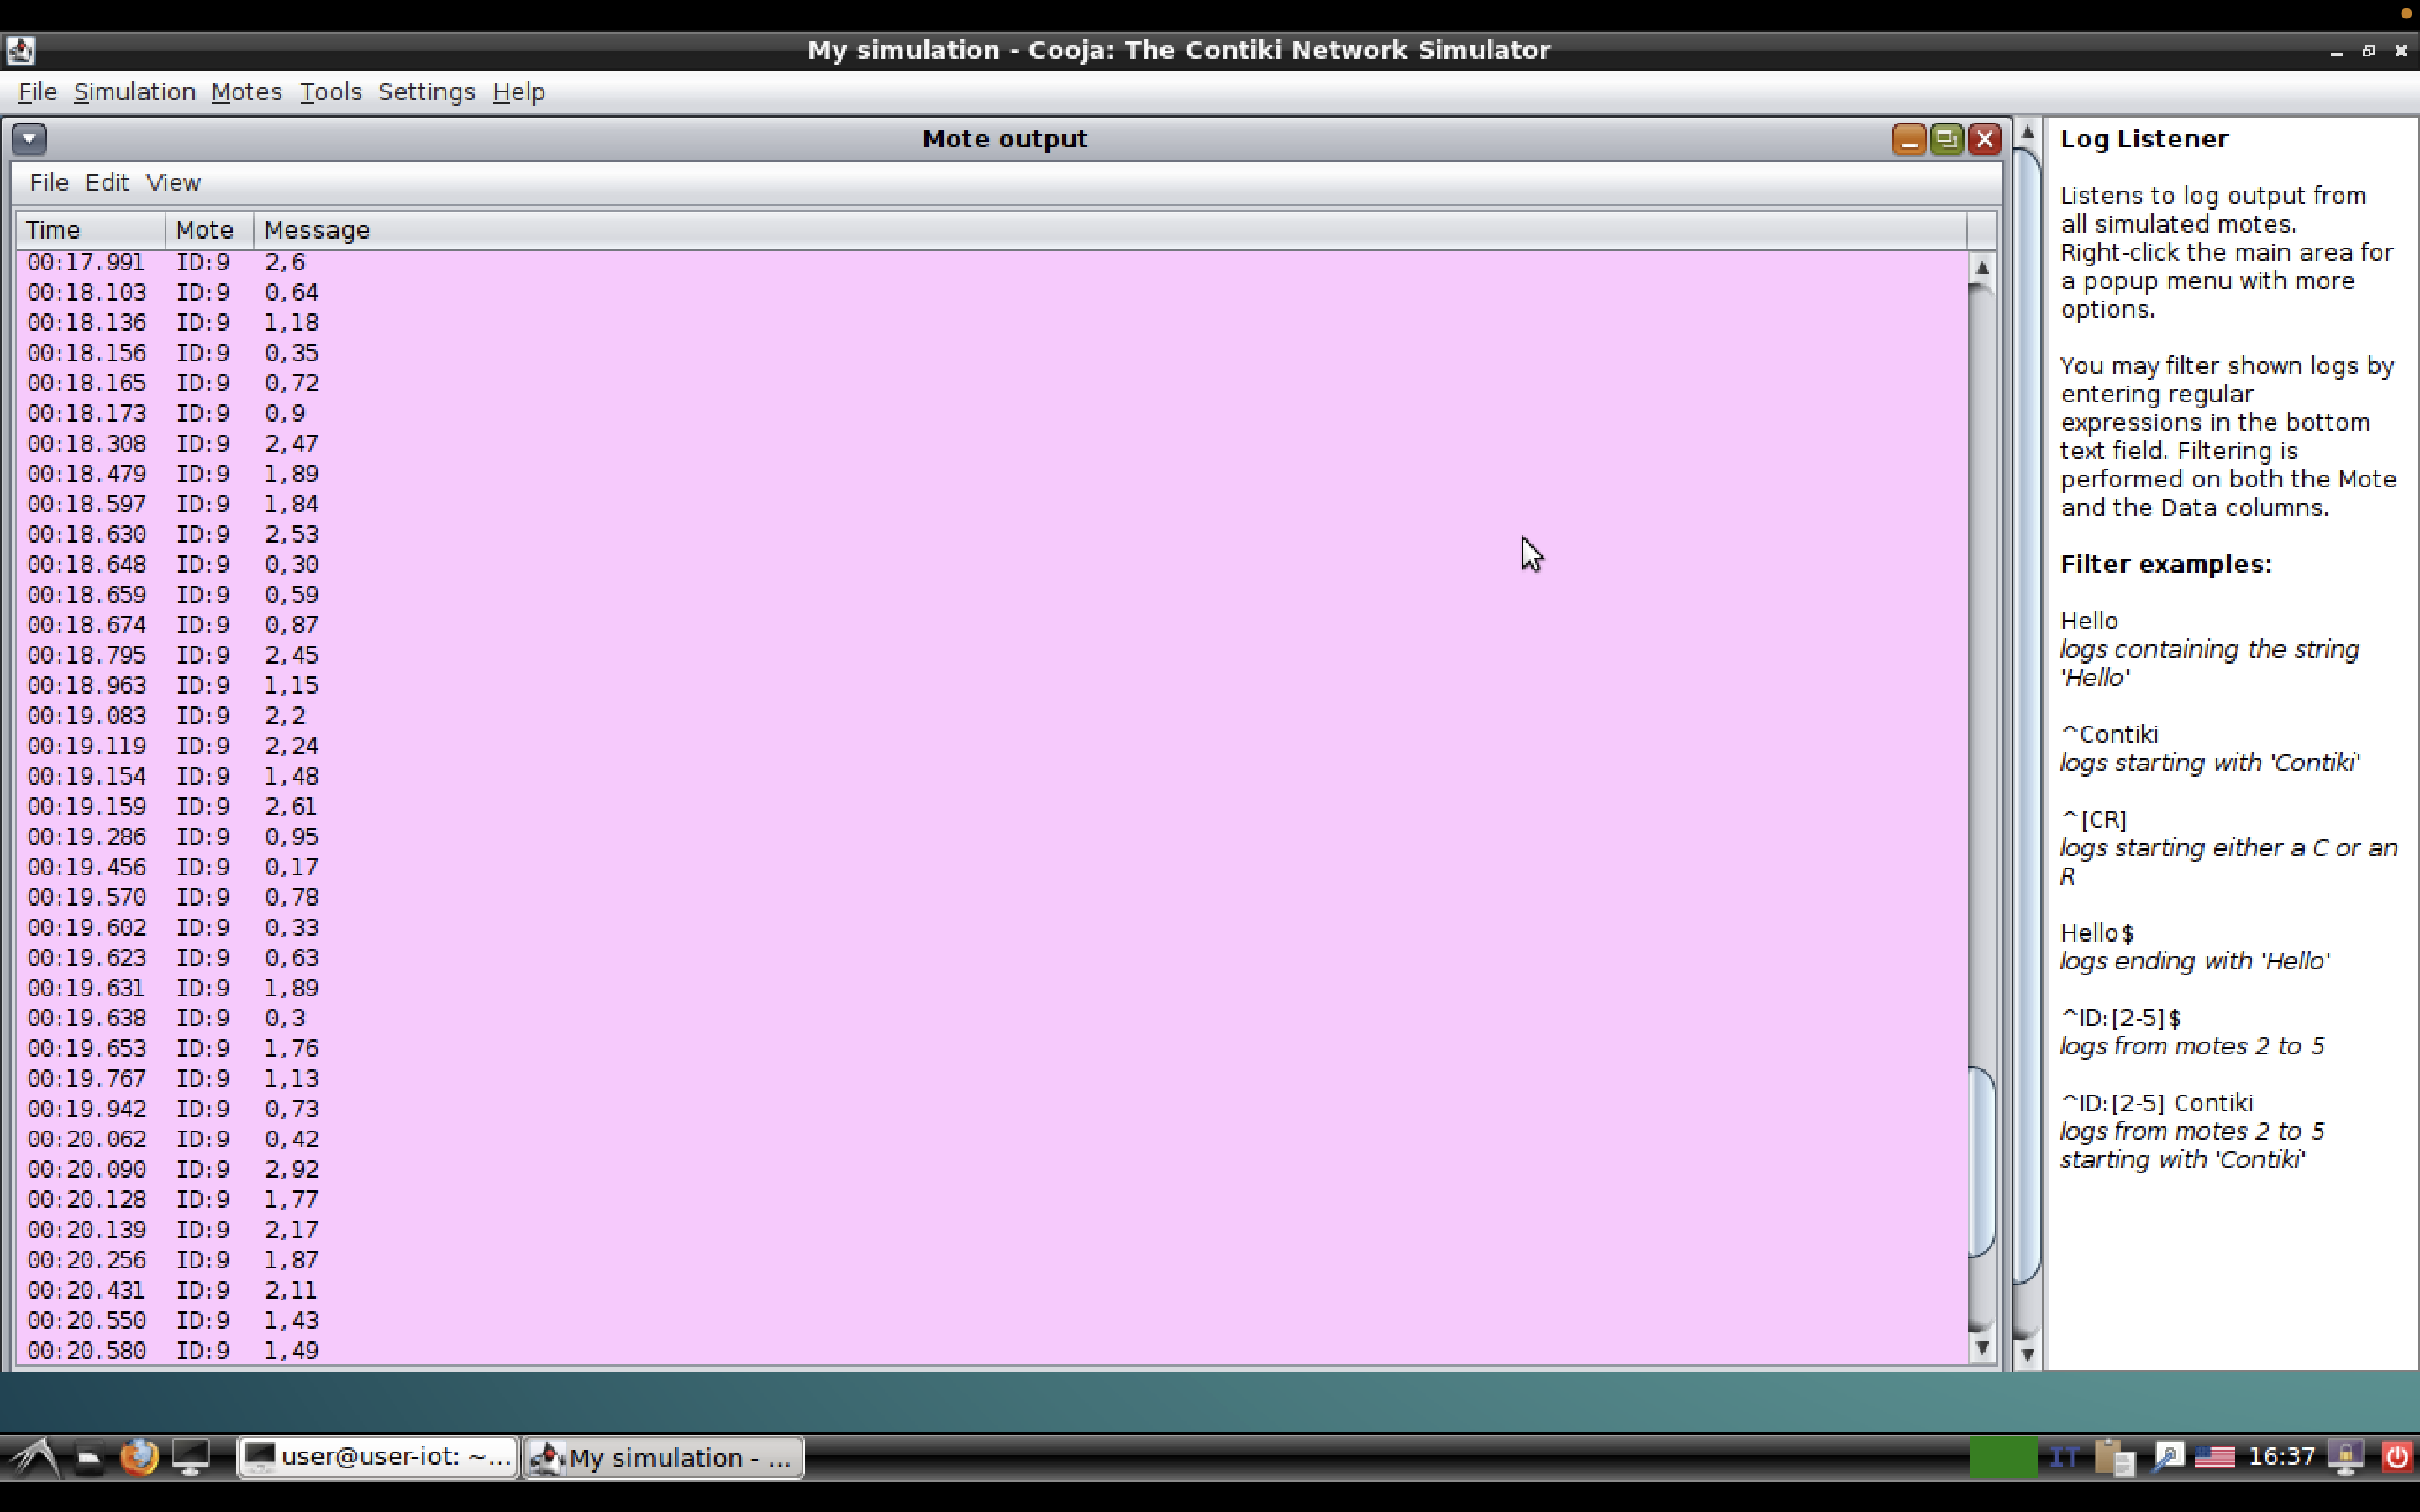
\includegraphics[width=1\textwidth]{images/publish_messages_cooja.png}
  \caption{Cooja log of publish messages sent by the PANC to Node-Red}
  \smallskip
  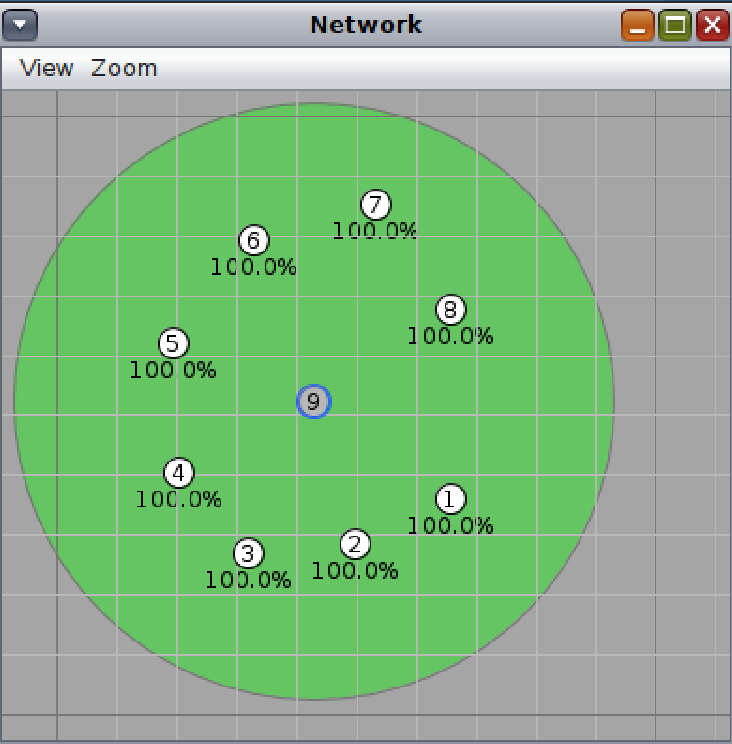
\includegraphics[width=0.6\textwidth]{images/network.png}
  \caption{Network topology}
  \medskip
  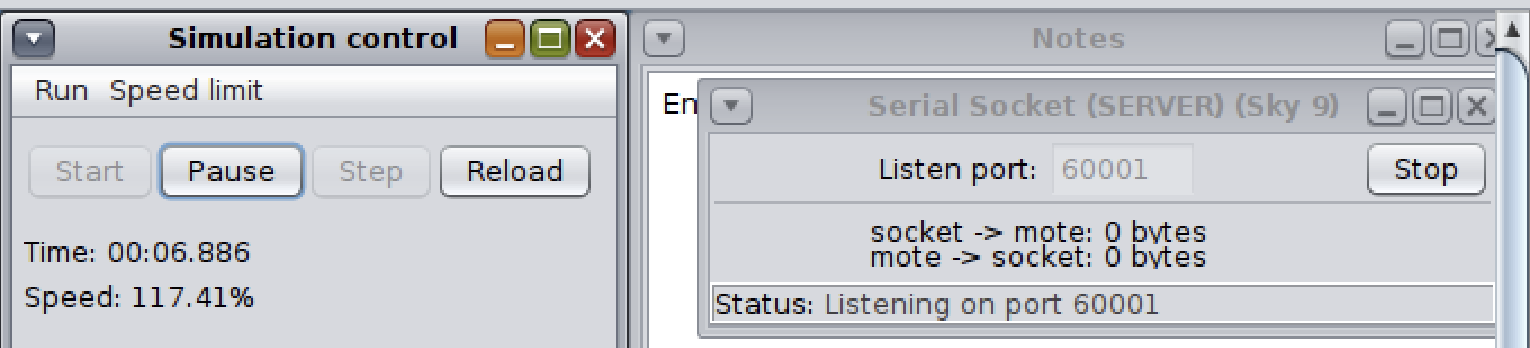
\includegraphics[width=0.6\textwidth]{images/serial_server_socket.png}
  \caption{Cooja simulation control and Serial Socket setup}
\end{figure}


\subsection*{Node-Red}
The Node-Red flow is indeed straighforward, it contains a network interface that intercept local input, 
and pass it towards the split function. Then the function divides the \texttt{PUBLISH} message in the 
form \texttt{Topic,Payload} to craft a proper MQTT publish request understandable by our 
\href{https://thingspeak.com/channels/2240116}{public ThingSpeak channel}, with 
topic \texttt{channels/channel\_id/publish} and payload \texttt{status=MQTTPUBLISH\&fieldX=data} 
\begin{figure}[h]
  \centering
  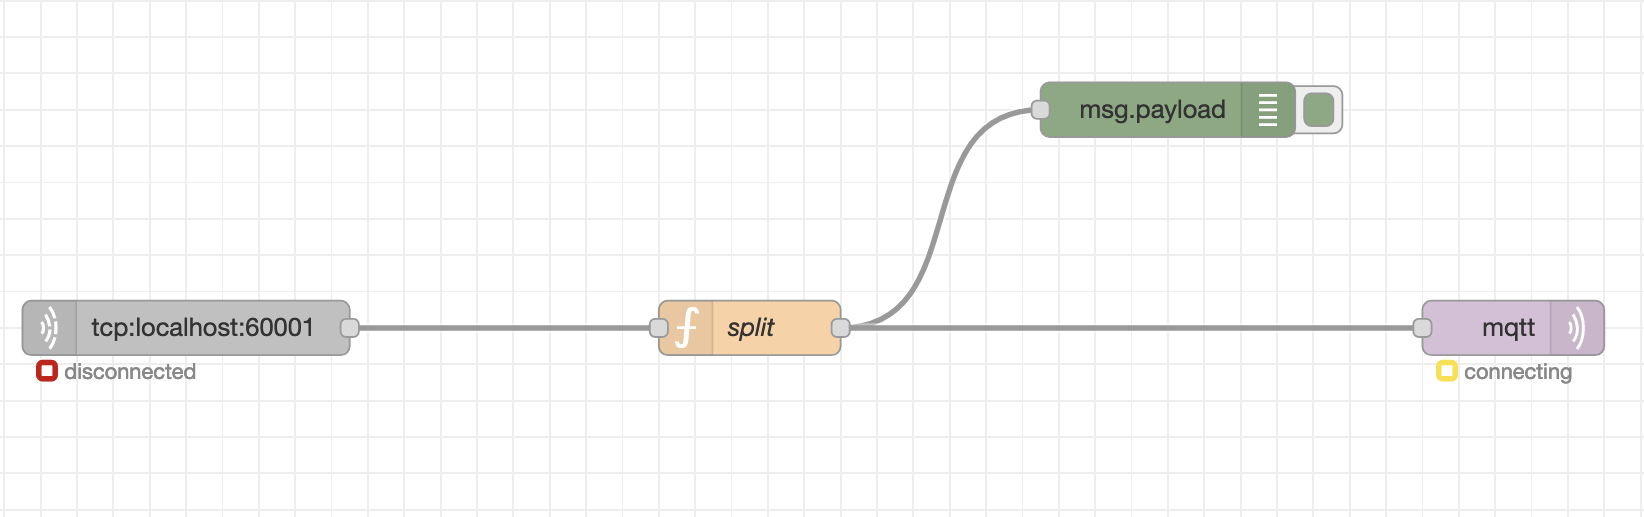
\includegraphics[width=1\textwidth]{images/node_red.png}
  \caption{Node-Red flow}
\end{figure}

\begin{figure}[h]
  \centering
  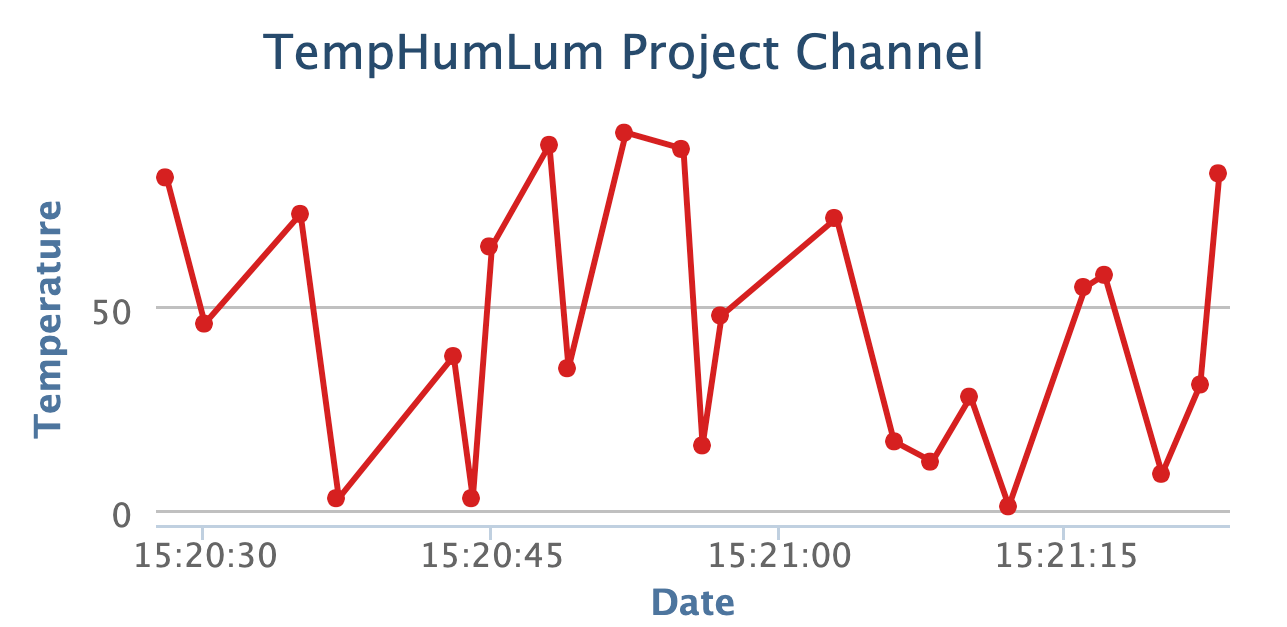
\includegraphics[width=0.6\textwidth]{images/temperature.png}
  \caption{Temperature chart}
  \medskip
  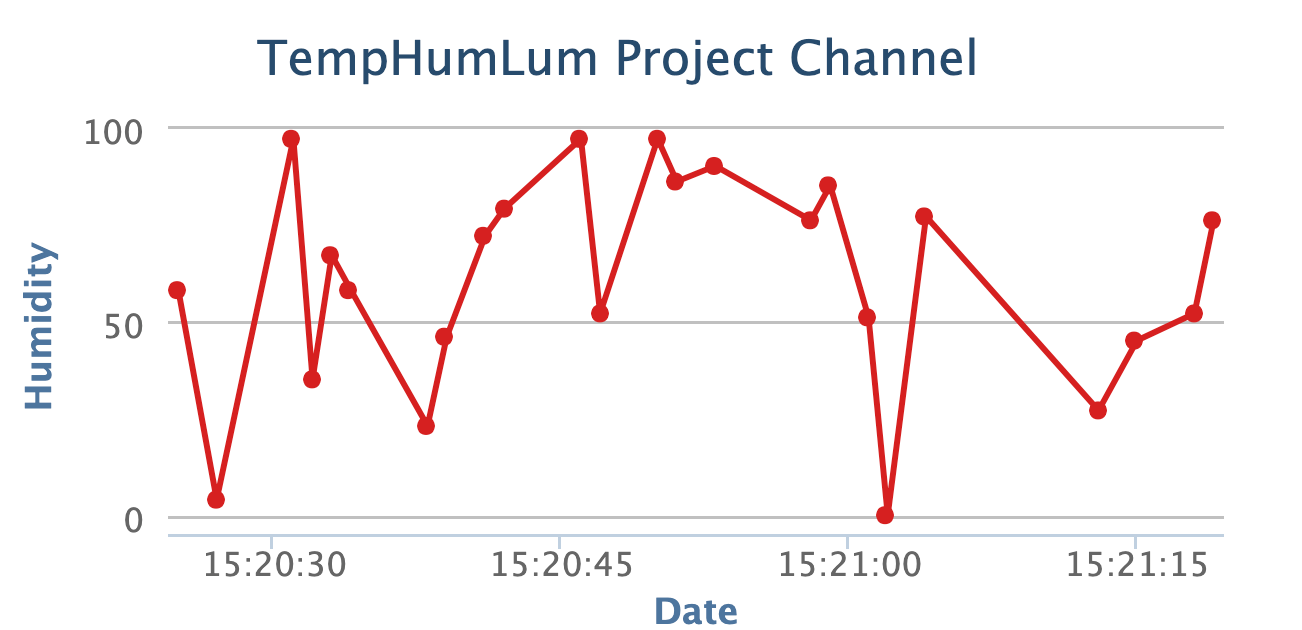
\includegraphics[width=0.6\textwidth]{images/humidity.png}
  \caption{Humidity chart}
  \medskip
  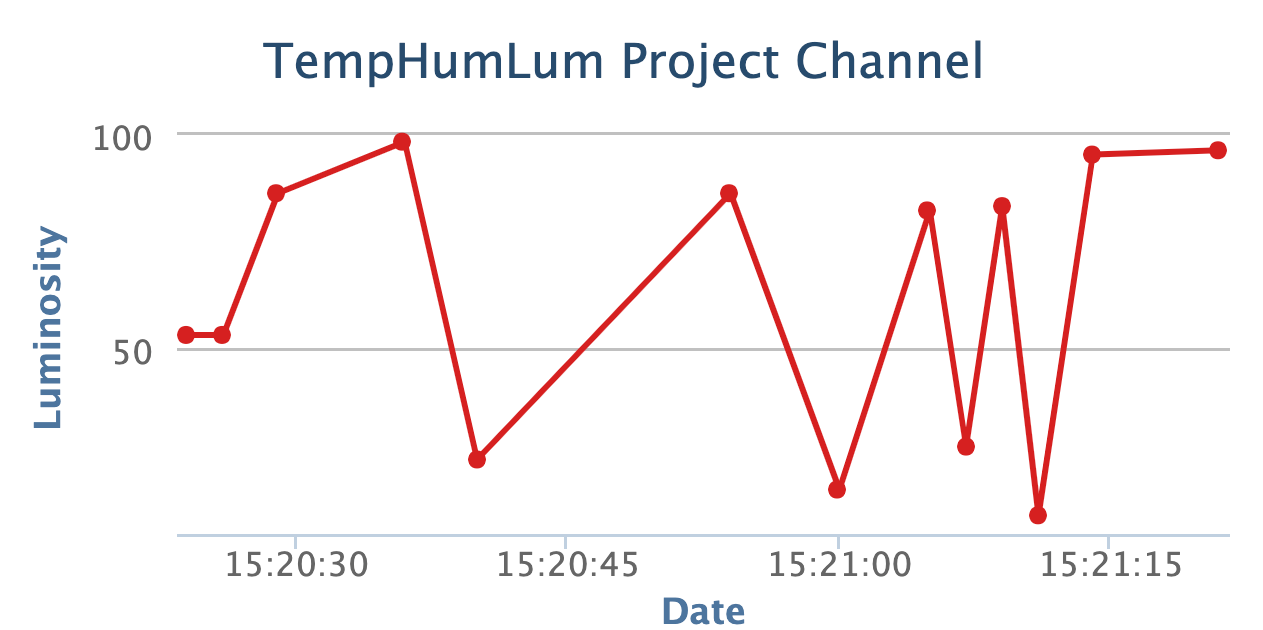
\includegraphics[width=0.6\textwidth]{images/luminosity.png}
  \caption{Luminosity chart}
\end{figure}


\end{document}
